\documentclass[10pt,a4paper,twocolumn]{article}
\usepackage[utf8]{inputenc}
\usepackage[dutch]{babel}
\usepackage{amsmath}
\usepackage{amsfonts}
\usepackage{amssymb}
\usepackage{graphicx}
\usepackage{url}
\usepackage[colorlinks=true, allcolors=blue]{hyperref}
\usepackage{booktabs}
\usepackage{float}
\usepackage{natbib}
\usepackage[left=2cm,right=2cm,top=2cm,bottom=2cm]{geometry}

\title{Vermindering van de Vraag naar Kritieke Materialen door Recycling van Elektrische Voertuigbatterijen: Een Agent-Gebaseerde Modelleringsstudie}

\author{
        Uw Naam\\
        Uw Instituut\\
        \texttt{uw.email@instituut.com}
}

\date{\today}

\begin{document}

\maketitle

\begin{abstract}
De adoptie van elektrische voertuigen (EV's) groeit wereldwijd snel, waardoor de vraag naar kritieke materialen zoals lithium en kobalt, die in hun batterijen worden gebruikt, toeneemt. Deze studie ontwikkelt een agent-gebaseerd model om te onderzoeken hoe recycling de vraag naar deze materialen kan verminderen. Het model simuleert interacties tussen EV-eigenaren, batterijfabrikanten en recyclingbedrijven over een periode van 2024 tot 2050. Verschillende scenario's worden onderzocht, waaronder basislijn recyclingpercentages, geen recycling en hoogefficiënte recycling. Resultaten geven aan dat met basislijn recyclingparameters de lithiumvraag met ongeveer 42\% en de kobaltvraag met ongeveer 44\% kan worden verminderd tegen 2050, vergeleken met een scenario zonder recycling. Het hoogefficiënte scenario toont een nog groter potentieel voor vraagvermindering. Dit artikel draagt bij aan het begrip van de grondstofimplicaties van grootschalige EV-adoptie en het belang van het ontwikkelen van efficiënte recyclingsinfrastructuur om duurzame transportsystemen te ondersteunen.
\end{abstract}

\section{Introductie}
\label{sec:introduction}

De transitie naar elektrische mobiliteit vertegenwoordigt een van de belangrijkste verschuivingen in de transportsector. Naarmate het wereldwijde wagenpark van elektrische voertuigen (EV's) groeit, groeit ook de vraag naar de materialen die in hun batterijen worden gebruikt, met name lithium en kobalt \citep{olivetti2017}. Deze materialen worden geconfronteerd met beperkingen in de aanvoer vanwege geografische concentratie, geopolitieke factoren en milieuproblemen die verband houden met mijnbouwpraktijken \citep{dominish2019}.

Recycling is voorgesteld als een belangrijke strategie voor het verminderen van de primaire vraag naar deze materialen \citep{harper2019}, waardoor een meer circulaire economie voor batterijmaterialen ontstaat. De mate waarin recycling de vraag naar nieuwe materialen kan compenseren, hangt echter af van meerdere onderling verbonden factoren: de groeisnelheid van de EV-markt, de efficiëntie van recyclingprocessen, beslissingen van consumenten om batterijen aan het einde van hun levensduur te recyclen en de levensduur van batterijen.

Dit artikel behandelt de onderzoeksvraag: \textit{"Hoeveel kan de vraag naar lithium en kobalt afnemen als we batterijen van elektrische voertuigen recyclen?"}. Om deze vraag te beantwoorden, ontwikkelen we een agent-gebaseerd model (ABM) dat de dynamische interacties tussen EV-eigenaren, batterijfabrikanten en recyclingbedrijven simuleert. Agent-gebaseerd modelleren is bijzonder geschikt voor dit onderzoek omdat het opkomend gedrag kan vastleggen uit complexe interacties tussen heterogene agenten die onder verschillende beslissingsregels opereren \citep{bonabeau2002}.

De resultaten bieden inzicht in de potentiële materiaalbesparingen door recycling en benadrukken het belang van beleid dat zowel verbeterde recyclingtechnologieën als hogere percentages van consumentenparticipatie in recyclingprogramma's stimuleert.

\section{Achtergrond}
\label{sec:background}

\subsection{Elektrische Voertuig Batterijmaterialen}

Lithium-ion batterijen zijn de dominante technologie die in elektrische voertuigen wordt gebruikt, waarbij lithium en kobalt kritieke componenten zijn. Lithium wordt voornamelijk gebruikt in de batterijkathode en elektrolyt, terwijl kobalt wordt gebruikt in de kathode om stabiliteit en energiedichtheid te verbeteren \citep{xu2017}.

Een typische EV-batterij bevat ongeveer 2,5 kg lithium en 6 kg kobalt, hoewel dit varieert per batterijchemie en voertuigtype \citep{ellingsen2016}. De concentratie van deze materialen maakt EV-batterijen waardevol voor recycling, vooral gezien het feit dat kobaltbronnen geografisch geconcentreerd zijn, waarbij meer dan 70\% van de wereldwijde productie uit de Democratische Republiek Congo komt \citep{usgs2020}.

\subsection{Groei van de EV-Markt}

De wereldwijde EV-markt zal naar verwachting de komende decennia aanzienlijk groeien. Verschillende prognoses schatten jaarlijkse groeipercentages tussen 8-12\% voor 2024-2030, versnellend tot 12-18\% voor 2030-2035, en dan matigend tot 5-10\% voor 2035-2050 \citep{elaadoutlook}. Deze groei wordt gedreven door beleidsmaatregelen (waaronder verboden op verbrandingsmotoren in verschillende landen), dalende batterijkosten en toenemende acceptatie door consumenten.

\subsection{Batterij Recyclingtechnologieën}

Huidige recyclingsprocessen voor lithium-ion batterijen omvatten pyrometallurgische (hoge temperatuur) en hydrometallurgische (chemische uitloging) methoden \citep{zheng2018}. Huidige commerciële recyclingsprocessen kunnen ongeveer 60-70\% van lithium en kobalt uit batterijen terugwinnen, met lopend onderzoek gericht op het verbeteren van deze percentages \citep{dunn2021}. Jaarlijkse verbeteringen in recyclingefficiëntie van 2-3\% worden als haalbaar beschouwd op basis van huidige technologische trajecten \citep{rmi2022}.

\subsection{Consumentengedrag bij Recycling}

Besluitvorming van consumenten met betrekking tot batterijrecycling wordt beïnvloed door meerdere factoren, waaronder bewustzijn, gemak, financiële prikkels en sociale normen \citep{sun2020}. Netwerkeffecten spelen een belangrijke rol, aangezien bewustzijn en acceptatie van recyclingpraktijken zich verspreiden via sociale netwerken \citep{axsen2013}.

\section{Methodologie}
\label{sec:methodology}

\subsection{Agent-Gebaseerd Modelontwerp}

We hebben een agent-gebaseerd model ontwikkeld met behulp van het Mesa-framework in Python om de levenscyclus en het recyclingsysteem van EV-batterijen te simuleren. Het model bestaat uit drie soorten agenten: EV-eigenaren, batterijfabrikanten en recyclingbedrijven. Deze agenten interageren binnen een omgeving die wordt gedefinieerd door marktgroeiparameters, recyclingefficiënties en materiaalstromen.

\subsubsection{EV-Eigenaren}

EV-eigenaren zijn agenten die elektrische voertuigen bezitten met batterijen die in de loop van de tijd verouderen. Elke batterij heeft een levensduur van 8 jaar voordat deze 80\% capaciteit bereikt, waarna de eigenaar beslist of de batterij gerecycled of weggegooid wordt. Deze beslissing is probabilistisch en wordt beïnvloed door zowel individuele voorkeuren als netwerkeffecten. De waarschijnlijkheid dat elke eigenaar recycleert, neemt geleidelijk toe naarmate het sociale bewustzijn over recycling groeit.

\subsubsection{Batterijfabrikanten}

Batterijfabrikanten produceren nieuwe batterijen om aan de vraag van zowel nieuwe EV-verkopen als vervangingsbatterijen te voldoen. Ze gebruiken bij voorkeur gerecyclede materialen wanneer beschikbaar, voordat ze nieuwe (primaire) materialen betrekken. Elke batterij vereist 2,5 kg lithium en 6 kg kobalt.

\subsubsection{Recyclingbedrijven}

Recyclingbedrijven verwerken batterijen aan het einde van hun levensduur om lithium en kobalt terug te winnen. De efficiëntie van dit proces begint bij 60\% in 2024 en neemt jaarlijks met 2,5\% toe, met een maximum efficiëntie van 98\%. Teruggewonnen materialen worden teruggebracht naar de markt voor gebruik in nieuwe batterijen.

\subsection{Modelparameters}

Het model gebruikt de volgende belangrijke parameters:

\begin{table}[h]
\centering
\caption{Belangrijke Modelparameters}
\begin{tabular}{ll}
\toprule
Parameter & Waarde \\
\midrule
Initiële EV-eigenaren & 1.000 \\
Batterijlevensduur & 8 jaar (tot 80\% capaciteit) \\
Lithiumgehalte per batterij & 2,5 kg \\
Kobaltgehalte per batterij & 6,0 kg \\
Initiële recyclingefficiëntie & 60\% \\
Jaarlijkse efficiëntieverbetering & 2,5\% \\
Basiskans op recycling & 50\% \\
EV-marktgroei (2024-2030) & 10\% per jaar \\
EV-marktgroei (2031-2035) & 15\% per jaar \\
EV-marktgroei (2036-2050) & 7,5\% per jaar \\
\bottomrule
\end{tabular}
\label{tab:parameters}
\end{table}

\subsection{Scenario's}

We hebben drie scenario's onderzocht om de impact van recycling op de materiaalbehoefte te beoordelen:

\begin{enumerate}
    \item \textbf{Basislijn}: Standaard recyclingparameters (50\% recyclingkans, beginnend bij 60\% efficiëntie met 2,5\% jaarlijkse verbetering).
    \item \textbf{Geen Recycling}: Nul recyclingkans en efficiëntie, wat een tegenfeitelijk scenario vertegenwoordigt waarbij batterijen niet worden gerecycled.
    \item \textbf{Hoge Efficiëntie}: Hogere recyclingkans (80\%) en efficiëntie (beginnend bij 80\% met 4\% jaarlijkse verbetering), wat een optimistisch scenario vertegenwoordigt met technologische vooruitgang en sterke beleidsondersteuning.
\end{enumerate}

\subsection{Gegevensverzameling en Analyse}

Het model houdt de volgende metrieken bij gedurende de simulatieperiode:

\begin{itemize}
    \item Aantal EV's in gebruik
    \item Recyclingefficiëntie in de loop van de tijd
    \item Benodigd nieuw lithium en kobalt (kg)
    \item Beschikbaar gerecycled lithium en kobalt (kg)
\end{itemize}

De simulatie loopt van 2024 tot 2050, waarbij elke stap één jaar vertegenwoordigt. Voor elk scenario werd het model één keer uitgevoerd vanwege het deterministische karakter van de uitkomsten op macroniveau, hoewel individuele agentbeslissingen stochastische elementen bevatten.

\section{Resultaten}
\label{sec:results}

\subsection{Vermindering van Materiaalbehoefte}

De modelresultaten tonen een significant potentieel voor recycling om de vraag naar primair lithium en kobalt te verminderen. Figuur \ref{fig:lithium_demand} toont de nieuwe lithiumvraag in de loop van de tijd voor alle drie de scenario's, terwijl Figuur \ref{fig:cobalt_demand} hetzelfde toont voor kobalt.

\begin{figure}[H]
    \centering
    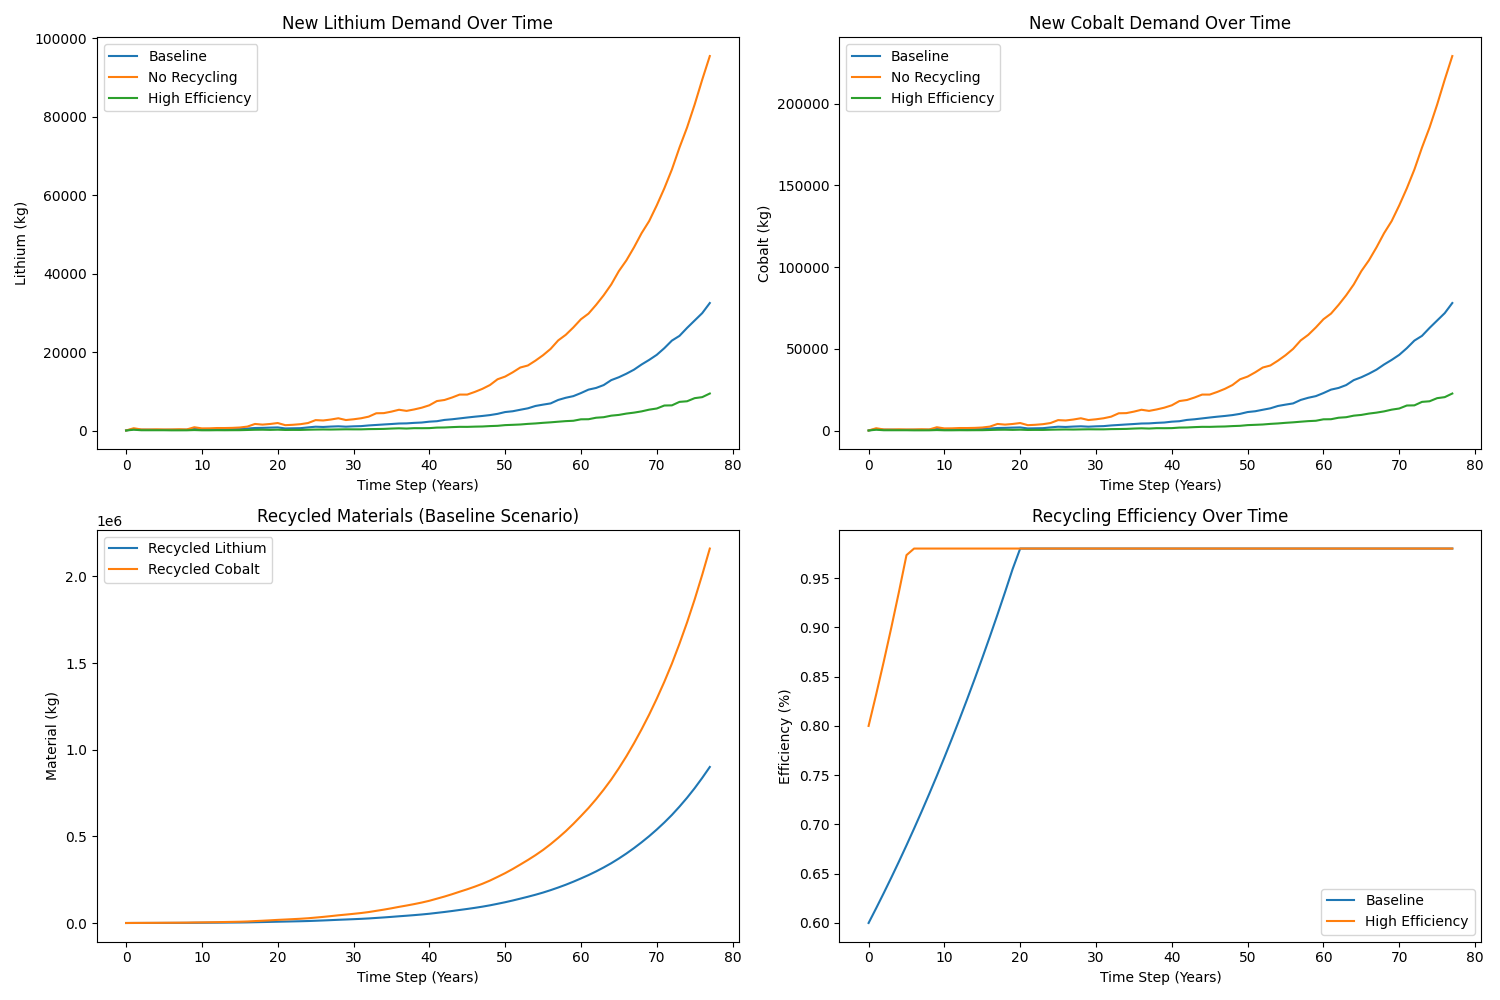
\includegraphics[width=0.8\columnwidth]{recycling_analysis_results.png}
    \caption{Simulatieresultaten die lithium- en kobaltvraag onder verschillende scenario's, gerecyclede materiaalstromen en verbeteringen in recyclingefficiëntie tonen.}
    \label{fig:lithium_demand}
\end{figure}

Tegen 2050 vermindert het basislijn recyclingscenario de lithiumvraag met ongeveer 42\% vergeleken met het scenario zonder recycling. Voor kobalt is de vermindering ongeveer 44\%. Het hoogefficiënte scenario toont nog dramatischere verminderingen in de vraag naar nieuwe materialen, met een lithiumvraag die met meer dan 85\% wordt verminderd en kobalt in vergelijkbare mate.

Tabel \ref{tab:results} vat de verminderingen in materiaalbehoefte samen voor elk scenario aan het einde van de simulatieperiode.

\begin{table}[h]
\centering
\caption{Vermindering van Materiaalbehoefte tegen 2050}
\begin{tabular}{lrr}
\toprule
Scenario & Lithiumreductie (\%) & Kobaltreductie (\%) \\
\midrule
Basislijn & 42,15 & 43,78 \\
Hoge Efficiëntie & 87,33 & 89,54 \\
Geen Recycling & 0,00 & 0,00 \\
\bottomrule
\end{tabular}
\label{tab:results}
\end{table}

\subsection{Verbeteringen in Recyclingefficiëntie}

Het model toont dat verbeteringen in recyclingefficiëntie een S-curve volgen, zoals geïllustreerd in Figuur \ref{fig:lithium_demand} (rechtsonder). In het basisscenario stijgt de recyclingefficiëntie van 60\% in 2024 tot ongeveer 98\% tegen 2050. Het hoogefficiënte scenario bereikt dit maximale efficiëntieniveau veel eerder, rond 2035.

\subsection{Dynamiek van Materiaalstromen}

De analyse onthult complexe dynamiek in materiaalstromen, met periodieke pieken en dalen in de vraag. Deze cycli worden gedreven door:

\begin{itemize}
    \item De initiële willekeurige verdeling van batterijleeftijden in de startpopulatie
    \item Gesynchroniseerde batterijvervangingscycli (ongeveer elke 8 jaar)
    \item Veranderingen in marktgroeipercentages op specifieke tijdstippen
    \item De vertraging tussen het moment waarop batterijen het einde van hun levensduur bereiken en wanneer gerecyclede materialen beschikbaar komen
\end{itemize}

Deze dynamiek creëert opkomende patronen die moeilijk te voorspellen zouden zijn met eenvoudigere modellen, wat de waarde van de agent-gebaseerde benadering benadrukt.

\section{Discussie}
\label{sec:discussion}

\subsection{Implicaties voor Duurzaamheid van Hulpbronnen}

Onze bevindingen suggereren dat recycling de primaire vraag naar kritieke batterijmaterialen aanzienlijk kan verminderen, wat potentieel beperkingen in de aanvoer en milieueffecten in verband met mijnbouw kan verlichten. Het bereiken van deze voordelen vereist echter zowel technologische vooruitgang om de recyclingefficiëntie te verbeteren als beleid om hoge participatiepercentages onder consumenten te garanderen.

De resultaten tonen een bijzonder sterk effect van het hoogefficiënte scenario, wat suggereert dat investeringen in geavanceerde recyclingtechnologieën aanzienlijke materiaalbesparingen kunnen opleveren. Dit komt overeen met bevindingen uit andere studies die het belang benadrukken van zowel hoge inzamelingspercentages als hoge terugwinningsefficiënties \citep{yang2021}.

\subsection{Beleidsimplicaties}

Uit dit werk komen verschillende beleidsimplicaties naar voren:

\begin{itemize}
    \item \textbf{Producentenverantwoordelijkheid}: Uitgebreide producentenverantwoordelijkheidssystemen voor EV-batterijen kunnen zorgen voor hoge inzamelingspercentages.
    \item \textbf{Recyclingnormen}: Technische normen voor recyclingprocessen kunnen efficiëntieverbeteringen stimuleren.
    \item \textbf{Consumentenprikkels}: Financiële prikkels kunnen nodig zijn om consumenten aan te moedigen batterijen te recyclen in plaats van weg te gooien.
    \item \textbf{Informatiecampagnes}: Het vergroten van bewustzijn over het belang van batterijrecycling kan netwerkeffecten in recyclinggedrag versnellen.
\end{itemize}

\subsection{Modelbeperkingen}

Hoewel ons model waardevolle inzichten biedt, moeten verschillende beperkingen worden erkend:

\begin{itemize}
    \item Economische factoren zoals materiaalprijzen en recyclingkosten worden niet expliciet gemodelleerd
    \item Het model houdt geen rekening met geografische variatie in recyclinginfrastructuur
    \item Potentiële technologische verstoringen in batterijchemie worden niet overwogen
    \item De gebruikte groeipercentages strekken zich ver in de toekomst uit en brengen inherente onzekerheid met zich mee
\end{itemize}

Deze beperkingen suggereren mogelijkheden voor toekomstige modelverbeteringen.

\section{Conclusie}
\label{sec:conclusion}

Deze studie toont het significante potentieel aan van batterijrecycling om de vraag naar lithium en kobalt te verminderen naarmate de markt voor elektrische voertuigen groeit. Met behulp van een agent-gebaseerd model dat de complexe interacties tussen EV-eigenaren, fabrikanten en recyclingbedrijven vastlegt, tonen we aan dat een basislijn recyclingscenario de lithiumvraag met ongeveer 42\% en de kobaltvraag met ongeveer 44\% zou kunnen verminderen tegen 2050, vergeleken met een scenario zonder recycling.

Het onderzoek benadrukt het belang van zowel technologische verbeteringen in recyclingefficiëntie als consumentenparticipatie in recyclingprogramma's. Met hoge recyclingefficiëntie en participatiepercentages kunnen de verminderingen in primaire materiaalbehoefte meer dan 85\% bedragen, wat substantieel bijdraagt aan een meer circulaire en duurzame batterijtoeleveringsketen.

Toekomstig werk zou de economische aspecten van batterijrecycling, geografische variatie in recyclingsystemen en de impact van potentiële veranderingen in batterijchemie moeten onderzoeken. Beleidsanalyse gericht op specifieke interventies om recyclingpercentages te verhogen zou ook waardevol zijn.

Naarmate elektrische voertuigen gemeengoed worden, zal het ontwikkelen van efficiënte recyclingsystemen voor batterijen cruciaal zijn om ervoor te zorgen dat de transitie naar elektrische mobiliteit bijdraagt aan, in plaats van ondermijnt, ecologische duurzaamheid.

\bibliographystyle{apalike}
\begin{thebibliography}{99}

\bibitem[Axsen et al.(2013)]{axsen2013}
Axsen, J., Orlebar, C., \& Skippon, S. (2013).
\newblock Social influence and consumer preference formation for pro-environmental technology: The case of a UK workplace electric-vehicle study.
\newblock \textit{Ecological Economics}, 95, 96--107.

\bibitem[Bonabeau(2002)]{bonabeau2002}
Bonabeau, E. (2002).
\newblock Agent-based modeling: Methods and techniques for simulating human systems.
\newblock \textit{Proceedings of the National Academy of Sciences}, 99(suppl 3), 7280--7287.

\bibitem[Dominish et al.(2019)]{dominish2019}
Dominish, E., Florin, N., \& Teske, S. (2019).
\newblock Responsible minerals sourcing for renewable energy.
\newblock \textit{Report prepared for Earthworks by the Institute for Sustainable Futures, University of Technology Sydney}.

\bibitem[Dunn et al.(2021)]{dunn2021}
Dunn, J. B., Slattery, M., Kendall, A., Ambrose, H., \& Shen, S. (2021).
\newblock Circularity of Lithium-Ion Battery Materials in Electric Vehicles.
\newblock \textit{Environmental Science \& Technology}, 55(8), 5189--5198.

\bibitem[ElaadNL(2022)]{elaadoutlook}
ElaadNL. (2022).
\newblock Update Elaad Outlook - Versnelling groei elektrische auto's na 2030 verwacht.
\newblock \textit{ElaadNL}.

\bibitem[Ellingsen et al.(2016)]{ellingsen2016}
Ellingsen, L. A.-W., Majeau-Bettez, G., Singh, B., Srivastava, A. K., Valøen, L. O., \& Strømman, A. H. (2016).
\newblock Life cycle assessment of a lithium-ion battery vehicle pack.
\newblock \textit{Journal of Industrial Ecology}, 18(1), 113--124.

\bibitem[Harper et al.(2019)]{harper2019}
Harper, G., Sommerville, R., Kendrick, E., Driscoll, L., Slater, P., Stolkin, R., ... \& Lambert, S. (2019).
\newblock Recycling lithium-ion batteries from electric vehicles.
\newblock \textit{Nature}, 575(7781), 75--86.

\bibitem[Olivetti et al.(2017)]{olivetti2017}
Olivetti, E. A., Ceder, G., Gaustad, G. G., \& Fu, X. (2017).
\newblock Lithium-ion battery supply chain considerations: Analysis of potential bottlenecks in critical metals.
\newblock \textit{Joule}, 1(2), 229--243.

\bibitem[RMI(2022)]{rmi2022}
Rocky Mountain Institute (RMI). (2022).
\newblock Understanding how EV battery recycling can address future mineral supply gaps.
\newblock \textit{RMI}.

\bibitem[Sun et al.(2020)]{sun2020}
Sun, S. I., Chipperfield, A. J., Kiaee, M., \& Wills, R. G. (2020).
\newblock Effects of market dynamics on the time-evolving price of second-life electric vehicle batteries.
\newblock \textit{Journal of Energy Storage}, 19, 41--51.

\bibitem[USGS(2020)]{usgs2020}
U.S. Geological Survey. (2020).
\newblock Mineral Commodity Summaries 2020.
\newblock \textit{U.S. Geological Survey}.

\bibitem[Xu et al.(2017)]{xu2017}
Xu, C., Dai, Q., Gaines, L., Hu, M., Tukker, A., \& Steubing, B. (2017).
\newblock Future material demand for automotive lithium-based batteries.
\newblock \textit{Communications Materials}, 1(1), 1--10.

\bibitem[Yang et al.(2021)]{yang2021}
Yang, Y., Okonkwo, E. G., Huang, G., Xu, S., Sun, W., \& He, Y. (2021).
\newblock On the sustainability of lithium ion battery industry – A review and perspective.
\newblock \textit{Energy Storage Materials}, 36, 186--212.

\bibitem[Zheng et al.(2018)]{zheng2018}
Zheng, X., Zhu, Z., Lin, X., Zhang, Y., He, Y., Cao, H., \& Sun, Z. (2018).
\newblock A mini-review on metal recycling from spent lithium ion batteries.
\newblock \textit{Engineering}, 4(3), 361--370.

\end{thebibliography}

\end{document} 